%% Citas verificadas contra el PDF; no hay marcadores [VERIFY] pendientes.

\section{MÉTODO}

Esta sección llama \emph{extensión} a la aplicación de navegador que recolecta del DOM los
datos con los que se resuelven las características, \emph{motor de riesgo} al conjunto de
servicios que derivan las características restantes y calculan el nivel estimado de riesgo, y
\emph{sistema} a la arquitectura completa, incluida la persistencia.

La unidad de análisis es una \emph{ficha de producto} que el comprador tiene abierta en su
navegador: el sistema no recorre catálogos ni consulta interfaces privilegiadas de la
plataforma, sino que opera sobre la misma información que el comprador ya tiene delante. Esta
restricción gobierna todas las decisiones de diseño que siguen. Separa esta propuesta de los
sistemas de detección desplegados por el operador del comercio \cite{ref28}.

\subsection{Características extraíbles del lado del cliente}

Para los efectos de esta arquitectura, se define como \emph{característica extraíble del lado
del cliente} a todo atributo de una publicación que cumpla tres condiciones simultáneas: ser
visible para el comprador antes del pago, residir en el documento ya entregado al navegador y
no requerir acceso a interfaces internas de la plataforma. La puntuación del producto, el
número de reseñas y el nombre de dominio cumplen estrictamente con estos criterios.

Esta distinción separa el presente trabajo de la línea dominante en detección de fraude, que
depende de la telemetría interna ya mencionada. El comprador dispone de un conjunto de
características restringido, por lo que la pregunta central que este trabajo aborda es si esos
datos accesibles resultan suficientes para producir una advertencia útil.

La definición se refiere al origen del dato, no al lugar donde se computa, y conviene separar
tres niveles que el resto del artículo mantiene distintos. El \emph{dato observado} lo lee la
extensión en el documento ya renderizado: la puntuación, la presencia de reseñas, el volumen de
ventas, la garantía anunciada, el medio de pago declarado y el nombre de dominio. La
\emph{característica derivada} la calcula el motor de riesgo a partir de ese dato o de otro
accesible públicamente, como ocurre con la veracidad de dominio, que parte del nombre de host y
consulta servicios de registro y resolución. La \emph{salida de modelo} es el valor que produce
un componente de aprendizaje automático, como la reputación del vendedor o la proporción
estimada de reseñas no auténticas. Las tres se apoyan en lo que el comprador tiene delante, y
ninguna exige telemetría interna de la plataforma; lo que cambia es dónde se computan, según
precisa la Tabla~\ref{tab:senales}.

\subsection{Lectura del DOM y recolección automatizada}

La operación que realiza la extensión requiere una caracterización precisa. Una revisión
sistemática define el \textit{web scraping} y el \textit{web crawling} como el proceso
automatizado de extracción de datos en el que las herramientas navegan a través de múltiples
páginas \cite{ref24}. La extensión propuesta no realiza ninguna de las dos operaciones: no
navega, porque es el usuario quien decide qué ficha abrir; no recorre múltiples páginas, porque
opera sobre el documento que el navegador ya renderizó. Su operación consiste en interpretar
contenido que ya le había sido entregado.

La misma revisión advierte que las herramientas apoyadas en selectores predefinidos son
susceptibles a cambios de maquetación, y que entre los desafíos del área figuran los riesgos
legales \cite{ref24}: lo primero se declara como amenaza a la validez más adelante, y lo
segundo es la razón para no retransmitir contenido de la plataforma más allá de las
características que el veredicto requiere.

\subsection{Protección de pago declarada}

Las plataformas de comercio de mayor tamaño publican esquemas mediante los cuales retienen el
pago hasta la conformidad del comprador o garantizan su devolución ante incumplimiento. Esa
declaración es un compromiso público y verificable en la propia ficha, y constituye por ello
una característica legítima. Su ausencia, en cambio, no es igualmente informativa: un vendedor
independiente puede ofrecer condiciones equivalentes sin anunciarlas, o anunciarlas donde la
extensión no alcanza a leer. Tratar el silencio como evidencia de inseguridad convertiría una
limitación del observador en una acusación sobre el observado, tanto más cuanto que las
contramedidas disponibles se despliegan y financian del lado del comercio \cite{ref30} y su
ausencia visible correlaciona con el tamaño del vendedor antes que con su honestidad.

La arquitectura se organiza en tres capas: cliente, motor de riesgo y persistencia. La
separación desacopla la observación del DOM, que ocurre en el navegador, del análisis de
riesgo, que requiere servicios externos, y de la persistencia, que sostiene la trazabilidad;
permite además sustituir los algoritmos de clasificación sin modificar la capa de observación.

\subsection{Capa cliente: observación sin recolección automatizada}

La capa cliente se implementa como una \emph{aplicación nativa en el navegador} (una
extensión) que se activa cuando el usuario abre una ficha de producto en una plataforma
soportada. La extensión recorre el árbol DOM ya renderizado, localiza mediante selectores los
elementos que exponen los atributos de interés precio, puntuación, número de reseñas,
identidad del vendedor, medios de pago anunciados, políticas de garantía y construye un
vector de observaciones que envía al motor de riesgo. Conviene ser preciso sobre el reparto:
la extensión no resuelve por sí sola las ocho características, sino que recolecta los datos
necesarios para resolverlas. Tres de ellas veracidad de dominio, reputación del vendedor y
autenticidad de reseñas las deriva el motor de riesgo, según detalla la
Tabla~\ref{tab:senales}, y la agregación del veredicto ocurre también allí. La extensión constituye el componente
principal de esta propuesta, y no por conveniencia de implementación. Es el único punto del
sistema que coincide, en espacio y en tiempo, con el instante en que el comprador decide.
Se ejecuta sobre la ficha que él tiene abierta, sin mediación de la plataforma y antes de que el
pago ocurra. Ningún otro componente de esta arquitectura coincide de ese modo con el
instante de la decisión.

Conviene precisar qué sale del navegador y qué no: salen los valores de los atributos leídos,
el nombre de host y el identificador de la publicación, por petición cifrada; no salen el
documento completo, el contenido de otras pestañas ni dato alguno de la sesión que el
comprador mantenga con la plataforma. La extensión no almacena datos sensibles del usuario.

Esta capa existe porque la advertencia que ha de llegar antes del pago debe producirla el
sistema y no el juicio del comprador \cite{ref27, ref3}. La ventaja técnica es que la
información necesaria ya fue entregada al navegador. El sistema no emite hacia la plataforma
del vendedor ninguna petición que el comprador no hubiera cursado en cualquier caso.

«Del lado del cliente» no significa, sin embargo, «sin servidor»: el vector observado viaja al
motor de riesgo, el analizador de dominio consulta servicios de registro, y cada consulta
queda registrada. La propuesta elimina la dependencia respecto de la plataforma del vendedor
a costa de introducir un nuevo tercero de confianza, con la política de retención y
anonimización que ello exige. Su otra contrapartida es la fragilidad ante cambios de
maquetación \cite{ref24}.

\subsection{Conjunto de características y regla de abstención ante evidencia ausente}

El motor de riesgo trabaja sobre ocho características, resumidas en la Tabla~\ref{tab:senales}.
Cada característica se define junto con la capa que la computa, su dominio de valores y   de
manera central para esta propuesta   el valor que toma cuando no puede determinarse.

\begin{table}[t]
\caption{Conjunto de características, origen y comportamiento ante evidencia ausente}
\label{tab:senales}
\centering
\footnotesize
\setlength{\tabcolsep}{3pt}
\renewcommand{\arraystretch}{1.15}
\begin{tabular}{@{}p{2.05cm}p{1.35cm}p{1.7cm}p{2.1cm}@{}}
\toprule
\textbf{Característica} & \textbf{Se computa en} & \textbf{Valores} & \textbf{Si no hay evidencia} \\
\midrule
Protección de pago declarada & Cliente & declarada / no declarada & \textit{no verificable} \\
Veracidad de dominio & Backend & escala ordinal & \textit{no verificable} \\
Reputación del vendedor & Backend & escala ordinal & \textit{no verificable} \\
Autenticidad de reseñas & Backend & proporción estimada & \textit{no verificable} \\
Puntuación del producto & Cliente & continua & ausente \\
Presencia de reseñas & Cliente & binaria & ausente \\
Políticas de garantía & Cliente & ordinal & \textit{no verificable} \\
Volumen de ventas & Cliente & entero & ausente \\
\bottomrule
\end{tabular}
\end{table}

La \emph{protección de pago declarada} fija el criterio que rige al resto. Plataformas como
MercadoLibre, Amazon o AliExpress declaran en la ficha que retienen el pago o que garantizan
la devolución ante incumplimiento, y la extensión detecta esa declaración; cuando no la
encuentra, el sistema no infiere que el pago sea inseguro sino que registra la característica
como \emph{no verificable}, según la distinción establecida en la subsección anterior.

Esta regla se aplica de manera uniforme: para toda característica se distingue entre valor
conocido, valor \emph{ausente} y valor \emph{no verificable}. Los dos últimos estados no son
intercambiables. Una característica es \emph{ausente} cuando el atributo no existe en la ficha
y esa inexistencia es en sí misma una observación: una publicación sin reseñas no tiene
puntuación del producto, y la lectura correcta no es que se ignore su valoración sino que no
ha sido valorada. Es \emph{no verificable} cuando el atributo puede existir pero el sistema no
logró comprobarlo: un vendedor independiente puede ofrecer garantía y no anunciarla en la
ficha, o el analizador de dominio puede no obtener respuesta del servicio de registro. El
primer estado informa sobre la publicación; el segundo, solo sobre los límites del observador.
Una característica se considera \emph{resuelta} cuando toma un valor conocido; los otros dos
estados la dejan sin resolver, y la Tabla~\ref{tab:senales} indica cuál adopta cada una cuando
la ficha no aporta evidencia. El agregador propaga esa distinción hasta el veredicto
mediante dos condiciones que deben cumplirse conjuntamente.

La primera es de cobertura. Sea $r$ el número de características resueltas de las ocho; el
sistema exige $r \geq 4$. El umbral mínimo se estableció para garantizar al menos una
característica por dimensión de riesgo (tres dimensiones) más una redundancia. Un umbral de
tres podría satisfacer la condición dimensional sin margen de error; uno de cinco reduciría
excesivamente los casos en que el sistema puede emitir un veredicto. La segunda es de
suficiencia por dimensión. Las ocho características cubren tres dimensiones de riesgo distintas:
la identidad del sitio (veracidad de dominio), la fiabilidad del vendedor (reputación, volumen
de ventas, políticas de garantía y protección de pago declarada) y la evidencia de la
comunidad (puntuación, presencia y autenticidad de reseñas). El sistema exige que al menos una
característica de cada dimensión se haya resuelto.

La elección de ocho características responde a la necesidad de cubrir las tres dimensiones con
más de un indicador en las dos primeras, lo que permite detectar inconsistencias y reducir la
influencia de valores atípicos. Es una decisión de diseño inicial y no un resultado: que ocho
basten, y que añadir más no aporte lo suficiente para justificar su costo de extracción, son
afirmaciones que requieren un análisis de ablación sobre datos reales, previsto para la etapa
siguiente.

Dos aspectos de esta regla quedan igualmente sujetos a verificación empírica. Los umbrales
$r \geq 4$ y $r \geq 6$ se eligieron por las razones expuestas, que no acreditan que sean los
valores adecuados: la Fase~1 de la Sección~IV, al medir qué se resuelve en fichas reales, es
la que permitirá ajustarlos. Y todas las características resueltas cuentan igual dentro de su
dimensión, supuesto discutible cuando una señal débil basta para dar por cubierta una
dimensión entera; ponderarlas por su confiabilidad es una alternativa que este trabajo deja
abierta.

Cuando ambas condiciones se satisfacen, el veredicto se emite con un nivel de confianza
derivado de la cobertura: alta si $r \geq 6$, media en caso contrario. Cuando alguna falla, el
sistema no emite riesgo sino \emph{evidencia insuficiente}, junto con la lista de
características que no pudo resolver.

La segunda condición distingue esta regla de un simple conteo: un umbral global trataría por
igual la pérdida de tres características redundantes y la de la única que informa sobre la
identidad del sitio, dejando al comprador sin protección frente a la suplantación. La
justificación de fondo es la asimetría de costos: presentar como seguro aquello que solo es
desconocido traslada al comprador un riesgo que el sistema no ha evaluado.

\subsection{Descomposición en servicios}

El motor de riesgo de la Fig.~\ref{fig:arquitectura} no es un bloque único: se despliega en
cuatro servicios desacoplados. Un analizador de veracidad de dominio verifica la legitimidad
del sitio web consultando registros DNS y patrones morfológicos; un analizador de reputación
evalúa el historial y las políticas del vendedor; una API de estimación de riesgo calcula el
nivel estimado de riesgo mediante un bosque aleatorio; y una API de detección de reseñas falsas
identifica contenido potencialmente fraudulento mediante un modelo DistilBERT. La API
centralizadora recibe las observaciones de la extensión, delega las características
relevantes a los cuatro servicios y agrega los resultados para emitir el veredicto. La
persistencia se resuelve sobre una base relacional que almacena las consultas y sus
resultados para trazabilidad y reentrenamiento. La separación responde a una propiedad que
el sistema necesita: cada servicio puede actualizarse de forma independiente cuando cambian
las características disponibles o los patrones lingüísticos del fraude, sin interrumpir el
servicio ni versionar la interfaz que consume la extensión.

\begin{figure}[!htbp]
\centering
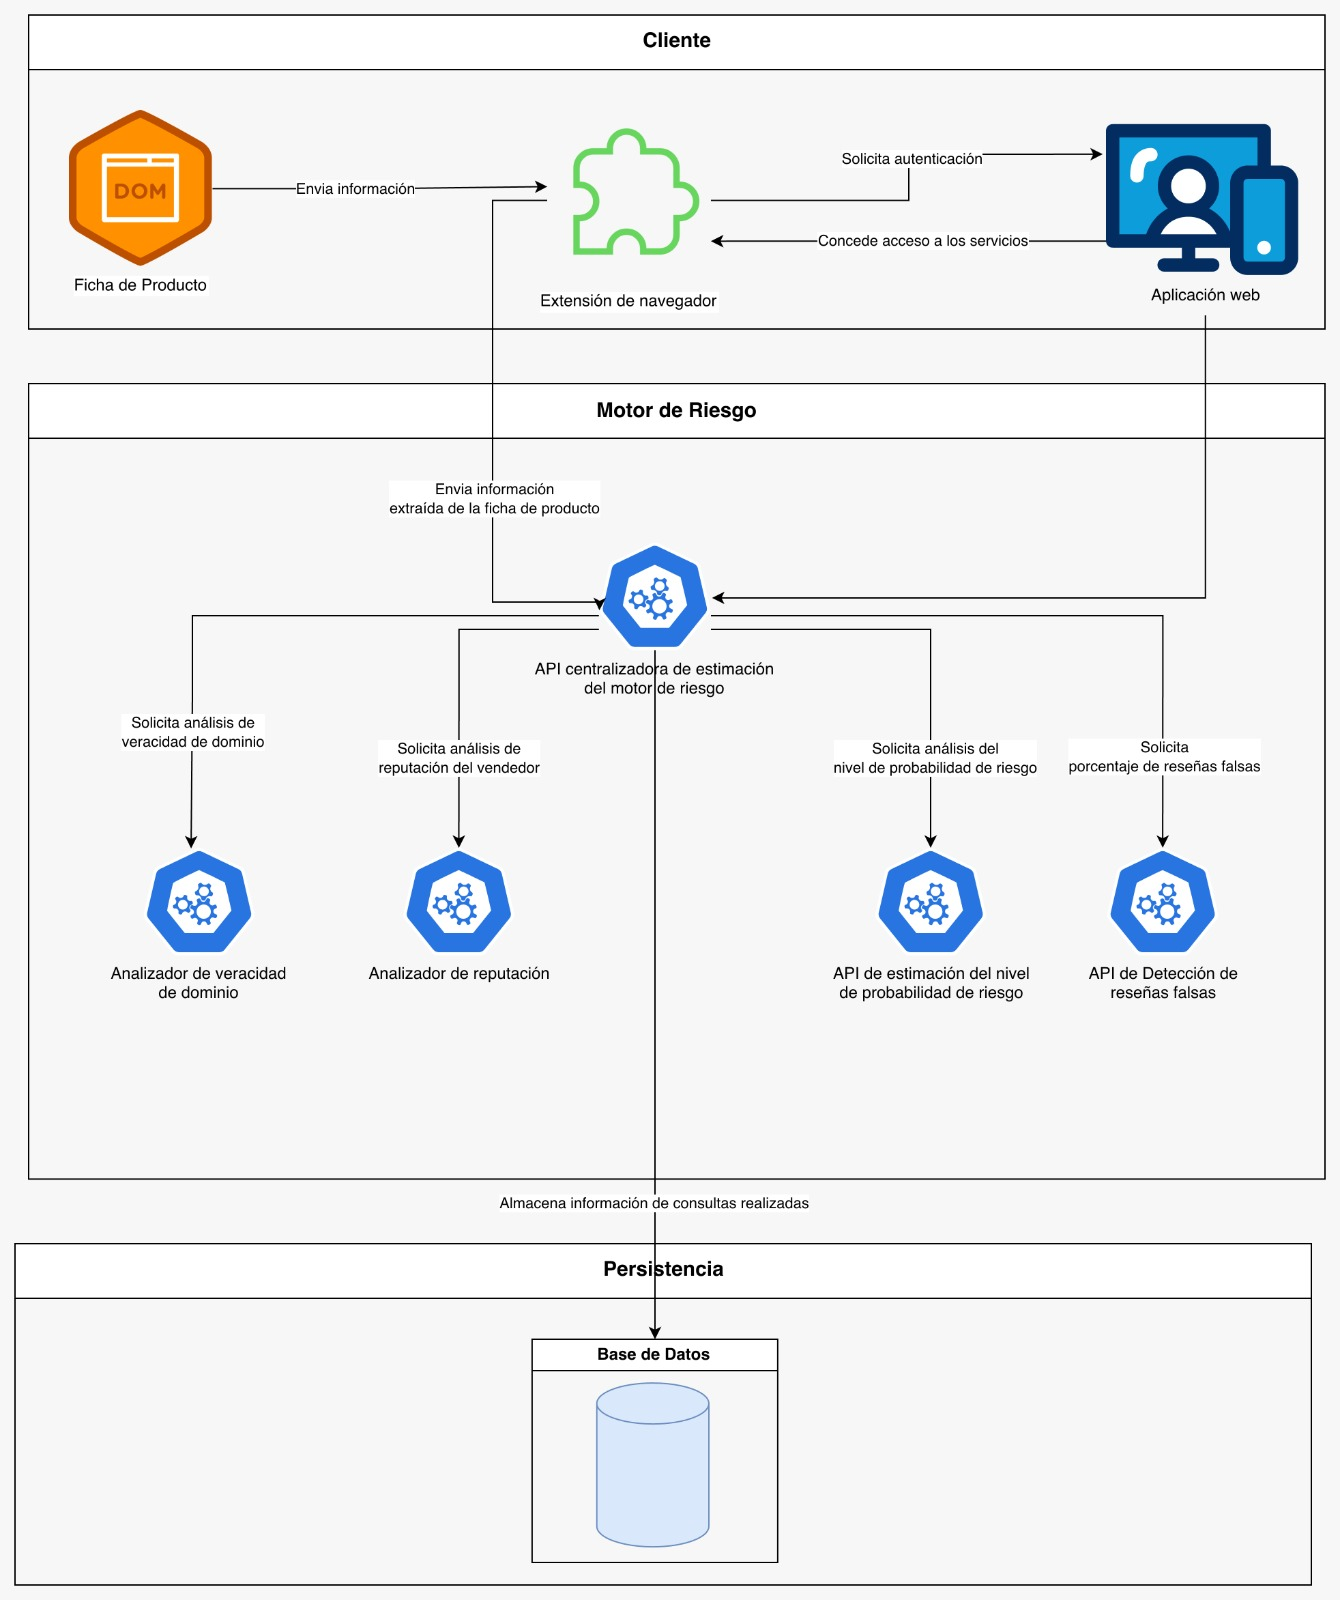
\includegraphics[width=\columnwidth]{figuras/arquitectura-logica.jpeg}
\caption{Arquitectura lógica propuesta. La capa cliente recolecta del DOM renderizado los
datos de las características y los envía a la API centralizadora del motor de riesgo, que se
descompone en cuatro servicios: analizador de veracidad de dominio, analizador de reputación,
API de estimación de riesgo y API de detección de reseñas falsas. La API centralizadora agrega
los resultados y almacena las consultas en la capa de persistencia.}
\label{fig:arquitectura}
\end{figure}

\subsection{Analizador de veracidad de dominio}

El analizador de dominio recibe el nombre de host de la ficha y devuelve una estimación
ordinal de veracidad. Se entiende aquí por \emph{veracidad de dominio} el grado en que el
dominio que aloja la ficha se corresponde con una operación establecida, y no con un despliegue
reciente o efímero de los asociados a la suplantación. Se expresa en una escala ordinal cuyo
nivel central se reserva a la ausencia de evidencia, de modo que un dominio sobre el que no se
obtuvo información no queda situado ni entre los confiables ni entre los sospechosos. Su
entrada se compone de atributos del registro del dominio, de la cadena de resolución incluidos
los registros de nombre canónico (CNAME) y de la coincidencia con patrones morfológicos
asociados a campañas de suplantación.

Este módulo es necesario porque ni el certificado SSL ni las listas de bloqueo del navegador
discriminan ya la suplantación \cite{ref25}. La ventaja de analizar registro y resolución en
lugar de contenido es que estos atributos aportan señales complementarias, menos dependientes
del contenido visible que el defraudador controla. Se ha mostrado que
características derivadas del registro permiten detectar URL de \textit{phishing} en dominios
aparcados \cite{ref7}, lo que sostiene la viabilidad del enfoque sobre esta clase de
atributos. El módulo no reemplaza la comprobación de
certificado, que la literatura de seguridad en comercio electrónico caracteriza como el
control fundacional y de menor costo \cite{ref30}, sino que la complementa en la dimensión
donde aquella dejó de ser informativa.

\subsection{Modelos de inferencia sobre vendedor y reseñas}

Dos componentes de aprendizaje automático completan el motor. El primero estima el riesgo del
vendedor a partir del vector de características extraídas y devuelve un nivel ordinal; el
segundo estima la proporción de reseñas presumiblemente fraudulentas en la ficha. La novedad
de la propuesta no reside en ellos, sino en cómo se integran sus salidas con las demás
características bajo la regla de la Sección~III-E, de modo que su configuración se documenta
solo en la medida en que hace reproducible el prototipo.

Para la estimación de riesgo del vendedor se emplea un bosque aleatorio y no una arquitectura
de mayor capacidad, por tres propiedades que el problema exige. La dimensionalidad: el vector
de entrada contiene ocho características heterogéneas   binarias, categóricas, discretas y
continuas   , un régimen en el que los métodos de ensamble por árboles operan sin normalización
ni codificaciones adicionales. La interpretabilidad: el modelo expone la contribución relativa
de cada característica. Y el costo: la inferencia sobre cien árboles es despreciable frente a
la latencia de red de la consulta. La elección responde por tanto a requisitos técnicos, y no
a una superioridad empírica sobre otras familias de algoritmos, extremo que los datos
disponibles no permiten arbitrar, como muestra la Sección~IV-A.

La interpretabilidad requiere una precisión, porque de ella depende la explicación que
acompaña al veredicto. La contribución relativa de las características que el bosque aleatorio
expone es una medida global, referida al modelo entero, y no explica por qué una publicación
concreta recibió el nivel que recibió. La explicación por caso exige un procedimiento distinto
importancia por permutación local, valores de Shapley o el recorrido de decisión del árbol
cuya elección este trabajo deja abierta y cuyo costo de cómputo debe medirse contra el tiempo
que el comprador espera.

El clasificador del que se dispone actualmente es un prototipo preliminar y no representa al
modelo del sistema propuesto: cien árboles entrenados sobre siete entradas, con 10\,000
registros sintéticos de tres clases equilibradas, partición 80/20 y semilla fija, sin la
veracidad de dominio que este trabajo incorpora. Añadirla exige reentrenar el modelo sobre un conjunto que la
contenga, y su ausencia es consecuencia de que este trabajo describe la arquitectura propuesta
y no una implementación ya construida.

El segundo componente estima la autenticidad de las reseñas con DistilBERT, un codificador
transformador destilado cuya configuración de ajuste recoge la tabla de configuración. La
elección de una variante destilada responde a una restricción operativa: la inferencia ocurre
entre la consulta de la extensión y la emisión del veredicto, de modo que su costo incide
sobre el tiempo que el comprador espera. Seis capas y 66.96 millones de parámetros reducen
ese costo frente a un codificador completo; la ejecución en precisión de 32 bits sobre unidad
central de proceso evita exigir aceleración por hardware. La contrapartida es una capacidad de
representación menor, cuya repercusión sobre la exactitud debe cuantificarse en la validación.

Su entrada no es únicamente el texto de la reseña: se serializan conjuntamente la categoría del
producto, la calificación asignada y el texto, porque una misma formulación puede resultar
verosímil o anómala según la calificación que la acompaña. El ajuste se realizó durante una
época, con tasa de aprendizaje de $2\times10^{-5}$, lotes de dieciséis secuencias de hasta 512
\textit{tokens} y dos clases. Este trabajo no evalúa el clasificador de reseñas: esa
configuración se declara para hacer reproducible el componente, no para respaldar afirmación
alguna sobre su desempeño. Ni el corpus de ajuste ni sus métricas de prueba forman parte de lo
reportado aquí, y la brevedad del ajuste es una limitación que su evaluación futura deberá
considerar.

La inferencia sobre reseñas es necesaria porque, según el resultado de equilibrio citado en
la Sección~II, la reputación visible es manipulable por construcción \cite{ref29}: tomar la
puntuación agregada como indicador de confianza coincide con el comportamiento que el vendedor
fraudulento busca inducir. La arquitectura incorpora por ello la estimación de autenticidad de
las reseñas como característica independiente de la puntuación, si bien la forma en que ambas
deben combinarse   y en particular si la segunda debe corregir a la primera antes de la
clasificación   constituye una decisión de diseño abierta que la validación deberá resolver.

\subsection{Agregación, presentación y persistencia}

El agregador combina las características resueltas en un veredicto con cuatro desenlaces
posibles: riesgo alto, moderado o bajo cuando la evidencia disponible permite decidir, y
\emph{evidencia insuficiente} cuando no. Los tres primeros se acompañan del nivel de confianza
y de la lista de características que los sustentan; el cuarto, de las características que no
pudieron resolverse. La presentación es deliberadamente explicativa: junto al veredicto se
muestra qué características se verificaron, cuáles quedaron indeterminadas y qué acredita cada
una, conforme al requisito de trazabilidad que la literatura de detección de fraude ha ido
incorporando frente a los clasificadores opacos \cite{ref28}.

La interfaz extiende el botón estándar del navegador: al abrirla, el comprador ve un indicador
de color con el veredicto, la lista de características verificadas con su valor y la de las no
resueltas con la razón de la falla.

Finalmente, cada consulta se registra en una base de datos junto con las características
extraídas y el veredicto emitido. El registro habilita la trazabilidad de cada advertencia y
constituye el conjunto de datos con el que los modelos se reentrenarán. Dado que la
información asociada a una consulta puede revelar hábitos de compra, el esquema se acota a lo
que esas dos funciones exigen: plataforma, identificador de la publicación, nombre de host,
valor y estado de cada característica, veredicto emitido y marca temporal. No se almacenan el
documento de la ficha, el texto de las reseñas ni la identidad del comprador cuando este usa
la extensión sin cuenta. La Sección~IV fija los términos de retención y disociación que rigen
durante la validación.